\chapter{Clean Architecture}
\label{ch:Clean_Architecture}

Die \textbf{Clean Architecture} hilft bei der Entwicklung von Systemen, die trotz externer Abhängigkeiten, wie zum Beispiel Frameworks, erweiterbar und flexibel sind.
Auch viele andere Entwurfsprinzipien verfolgen dieses Ziel.
Die Clean Architecture beschreibt dabei aber Prinzipien auf einer höheren Ebene, als zum Beispiel die SOLID-Prinzipen, die ähnliche Ziele verfolgen.
Bei der Clean Architecture wird das System in mehrere Schichten aufgeteilt, die häufig als konzentrische Kreise dargestellt werden.
Abbildung \ref{fig:clean_architecture_circles} zeigt die originale Darstellung der Clean Architecture.
\begin{figure}[h]
    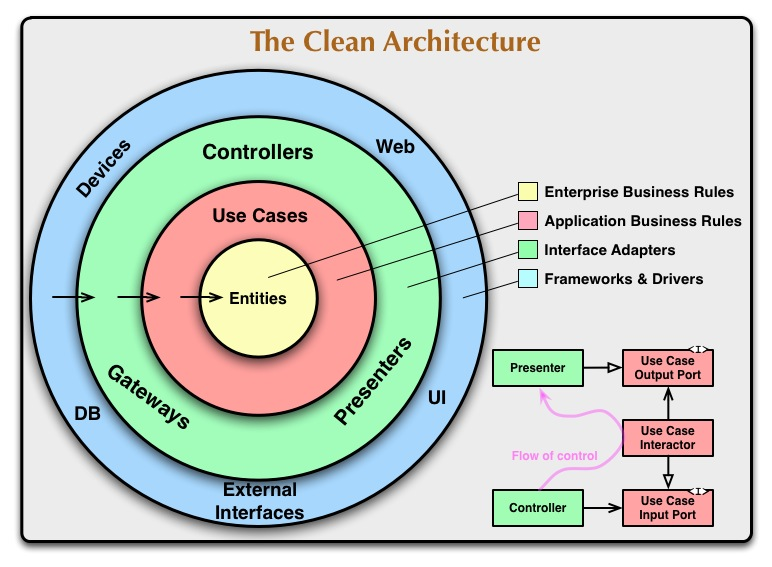
\includegraphics[width=15cm]{clean_architecture.jpg}
    \centering
    \caption{Darstellung der Clean Architecture \cite{martin_clean_architecture}}
    \label{fig:clean_architecture_circles}
\end{figure}


Der innere Kreis repräsentiert dabei den Kern der Anwendung.
Weiter außen liegende Kreise sind konzeptuell weiter vom Kern der Anwendung entfernt.
Zum Beispiel werden Benutzerschnittstelle, Datenbank, Frameworks und ähnliches zum äußersten Kreis zugeordnet.

Die Grundlage der Clean Architecture ist die sogenannte \textbf{Dependency Rule}.
Nach dieser Regel dürfen Abhängigkeiten nur zu weiter innen liegenden Schichten existieren und nicht umgekehrt.
Dadurch bleiben die inneren Schichten komplett unabhängig von den äußeren Schichten und diese wiederum werden leicht austauschbar.
Zur Umsetzung der Regel können Schnittstellen in inneren Schichten definiert, und in äußeren implementiert werden (siehe dazu auch \textit{\hyperref[sec:DIP]{Dependency Inversion Principle}}).

Die \textit{Interface Adapters}-Schicht (oder auch Adapter-Schicht) aus Abbildung \ref{fig:clean_architecture_circles} hat den Zweck, externe Abhängigkeiten möglichst von der eigentlichen Anwendung zu trennen.
In dieser Schicht werden vor allem Datenkonvertierungen von internen zu externen Formaten und umgekehrt durchgefürht.
Das System kann dadurch intern mit einem beliebigen Format arbeiten und ist dementsprechend unabhängig von Datenformaten, die von externen Abhängigkeiten benötigt werden.
Wenn zum Beispiel die Datenbank ausgetauscht werden soll reicht es aus, einen neuen Adapter zu implementieren.
Die eigentliche Kernanwendung muss also nicht verändert werden, wenn externe Komponenten ausgetauscht werden sollen.
Damit ist die Entwicklung flexibler und möglichst technologieunabhängiger System möglich.
Es gilt zu beachten, dass die gezeigten vier Schichten keine feste Vorgabe, sondern vielmehr ein Beispiel für eine mögliche Aufteilung sind.
In realen Anwendungsfällen kann die Struktur durchaus abweichen, solange die Dependency Rule eingehalten wird \cite{martin_clean_architecture}.

\section{Begründung der Clean Architecture}
Beim Entwurf der Architektur des vorliegenden Projekts wurde nicht bewusst auf die Clean Architecture geachtet, was an der Struktur des Projekts erkennbar ist.
Anstatt die Anwendungen in mehrere Packages aufzuteilen um abgegrenzte Schichten deutlich zu machen, sind die Klassen nur nach Verantwortlichkeit gruppiert in Packages aufgeteilt.
Da die Verantwortlichkeiten allerdings nicht immer einer einzelnen Schicht zugeordnet werden können, ist diese Gruppierung unzureichend.
Die Analyse der Clean Architecture in diesem Projekt wird durch diese Tatsache und vor allem auch durch den Anwendungsbereich des Systems deutlich erschwert.
Dadurch, dass das System darauf ausgelegt ist, Daten einer externen API zu verarbeiten, ist eine relativ starke Abhängigkeit zu dieser API unumgänglich.

Trotzdem wurde darauf geachtet, unnötige Abhängigkeiten zu vermeiden und das System so flexibel wie möglich zu gestalten.
Da die Konzepte der Clean Architecture bei Beginn der Entwicklung nicht bekannt waren, folgt das Design nicht immer den Grundlagen der Clean Architecture und die Zuordnung von Klassen zu Schichten fällt schwer.
Dennoch können grobe Schichten identifiziert werden.
Das User-Interface wird zum Beispiel in einem eigenen Package zusammengefasst und der Rest der Anwendung hat keinerlei Abhängigkeiten zu den Klassen der Oberfläche.
An anderen Stellen werden wiederum Defizite deutlich.
Im \textit{client}-Package zum Beispiel befinden sich sowohl Interfaces, die der Kernanwendung zuzuordnen sind, als auch Klassen, die konkrete Implementierungsdetails mit starren Abhängigkeiten zu externen Libraries sind.
Konkret sind die Interfaces \textit{UserContributionsClient} und \textit{RepositoryDataClient} Teil der Kernanwendung, da sie wichtige Funktionalität der Anwendung abstrahieren.
Andererseits implementiert die Klasse \textit{GithubOAuthClient} diese Interfaces und ist sehr Technologiespezifisch und ist Abhängig von einer konkreten Bibliothek.
Trotzdem können auch hier die Grundideen der Clean Architecture erkannt werden, da innerhalb der Kernanwendung immer mit den Abstraktionen der Interfaces gearbeitet wird, anstatt die konkrete Implementierung zu verwenden, die Implementierung ist dadurch also austauschbar.

\subsection{Fazit Clean Architecture}
Bei der Betrachtung der Architektur des Systems ist die Umsetzung Clean Architecture nicht direkt ersichtlich, da sie nicht explizit beachtet wurde.
Trotzdem wird bei genauerer Analyse deutlich, dass zumindest das Grundprinzip der Clean Architecture - die Dependency Rule - meist umgesetzt wurde, auch wenn dabei nicht immer klar ist, wo die Grenzen der einzelnen Schichten verlaufen.
Um das Design des Systems zu verbessern sollten die Schichten klar definiert und voneinander abgegrenzt werden.
Die Aufteilung auf Schichten muss dann unbedingt an der Projektstruktur deutlich werden, sodass die weitere Arbeit an diesem System einfach ist.
